\documentclass[a4paper,10pt]{report}
\usepackage[utf8]{inputenc}
\usepackage{graphicx}
\usepackage{verbatim}
\usepackage[framed,numbered,autolinebreaks,useliterate]{mcode}
\usepackage{ctable} % for \specialrule command

\usepackage[a4paper, total={6in, 8in}]{geometry}
% Title Page
\title{\textbf{OPTICAL COMMUNICATION COMPONENTS \\ Lab 4}}
\author{Nicola Simoni, Tadewos Somano, Melkamsew Tenaw}
\date{University of Brescia, Faculty of Engineering\\A.Y. 2013-2014}


\begin{document}
\maketitle


%%%%%%%%%%%%%%%%%%%%%%%%%%%%%%%%%%%%%%%%%%%%%%%%%%%%%%%%%%%%%%%%%%%%%%%%%%%%%%%%%%%%%%%%%%%%%
\section*{Exercise 1}
Following is reported our Matlab BPM code that solves the NLSE:
\lstinputlisting{BPM.m}
As test we set the following parameters:
\begin{itemize}
 \item $\alpha = 0$
 \item $\gamma = 0$
 \item $\beta_2 = -5 \cdot 10^{-27} \ [s^2/m]$
 \item $\lambda = 1.55 \mu m$
\end{itemize}
and we simulate the propagation of the following Gaussian pulse, over a distance of 40 Km:
\begin{equation}\label{pulse}
A(T)=A_0 \cdot e^{-\frac{1}{2}\cdot (\frac{T}{T_0})^2}
\end{equation}

with $A_0=1$ and $T_0=1.25 \cdot 10^{-11} \ s$.
In Figure \ref{es1} is shown the simulation result.

\begin{figure}[!ht]
  \centering
  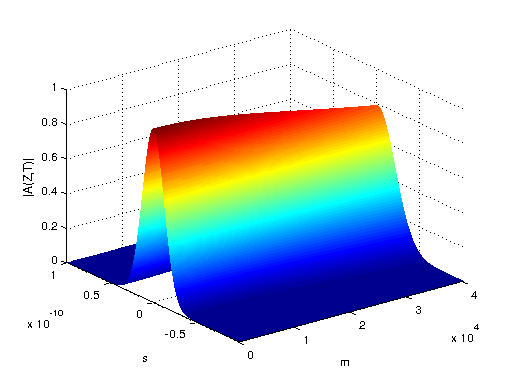
\includegraphics[width=11cm]{es1.png}\\
  \caption{Propagation of the Gaussian pulse $A(T)$.}
  \label{es1}
\end{figure}

\newpage
%%%%%%%%%%%%%%%%%%%%%%%%%%%%%%%%%%%%%%%%%%%%%%%%%%%%%%%%%%%%%%%%%%%%%%%%%%%%%%%%%%%%%%%%%%%%%%
\section*{Exercise 2}
Following is reported the procedure to derive the explicit evolution equation for the chirp $C_1(L)$.
The pulse at distance L has the following form:
\begin{equation}\label{c1_1}
 A(L,T)=A_0 \cdot \alpha_L \cdot e^{-\frac{1+i C_1}{2} \left(\frac{T}{T_0}\right)^2}
\end{equation}
that can also be written as:
\begin{equation}\label{c1_2}
 A(L,T)=\frac{A_0}{R(L)} \cdot e^{-\frac{1+i C}{2} \left(\frac{T}{T_0}\right)^2\frac{1}{R(L)^2}}
\end{equation}
where $$R(L)=\sqrt{1+(C-i)\beta_2 L/{T_0}^2}$$

To compute $C_1(L)$ we have to match the imaginary and the real part of equations (\ref{c1_1}) and (\ref{c1_2}).
We substitute R(L) in equation (\ref{c1_2}) and we rearrange the exponent, in order to separate the real and the imaginary parts:

$$\frac{(1+iC)T^2}{2{T_0}^2(1+(C-i)\beta_2L/{T_0}^2)}=\frac{(1+iC)T^2}{2({T_0}^2+\beta_2 C L-i\beta_2 L)}=\cdots$$
$$\cdots=\frac{(1+iC)T^2({T_0}^2+\beta_2 C L + i\beta_2 L)}{2(({T_0}^2+\beta_2 C L)^2+(\beta_2 L)^2)}
=\frac{T^2 {T_0}^2 + i T^2 (\beta_2 L + C {T_0}^2 + C^2 \beta_2 L)}{2(({T_0}^2+\beta_2 C L)^2+(\beta_2 L)^2)}
$$

the imaginary part is (with a change of sign):
$$\frac{T^2(\beta_2 L + {C T_0}^2 + C^2  \beta_2 L)}{2(({T_0}^2+\beta_2 C L)^2+(\beta_2 L)^2)}$$

and we can equate it to the imaginary part of equation (\ref{c1_1}), obtaining:
\begin{equation}\label{c1_3}
 \frac{C_1}{2} \left(\frac{T}{T_0}\right)^2=\frac{T^2(\beta_2 L + {C T_0}^2 + C^2  \beta_2 L)}{2(({T_0}^2+\beta_2 C L)^2+(\beta_2 L)^2)}
\end{equation}

from the comparison of the real part of equation (\ref{c1_1}) with the real part of equation (\ref{c1_2}), we obtain:
$$\frac{1}{2}\left(\frac{T}{T_0}\right)^2=\frac{T^2 {T_0}^2}{2(({T_0}^2+\beta_2 C L)^2+(\beta_2 L)^2)}$$
substituting this value in equation (\ref{c1_3}) we obtain the final result:

$$C_1 = \frac{T^2(\beta_2 L + {C T_0}^2 + C^2 L \beta_2)}{T^2 {T_0}^2}$$

that is:
\begin{equation}\label{c1_end}
 C_1(L)=C+(1+C^2)\beta_2 L / {T_0}^2
\end{equation}


We compute $C_1(L)$ using equation (\ref{c1_end}) for the following values of length: L/4, L/2, 3/4L, L and for C equal to 0, -2, 2.
L is the dispersion distance and it is defined as $L=L_D={T_0}^2/|\beta_2|$
(in this case $T_0=1.25 \cdot 10^{-11} \ s$ and $\beta_2 = -5 \cdot 10^{-27} \ [s^2/m]$).

\begin{table}[ht!]
  \begin{center}
    \begin{tabular}{ccccc}
      \specialrule{.1em}{.05em}{.05em}
	  & $C_1(L/4)$ & $C_1(L/2)$ & $C_1(3/4L)$ & $C_1(L)$\\
	 \hline
	C=0 & -0.25 & -0.5 & -0.75 & -1\\
	C=2 & 0.75 & -0.5 & -1.75 & -3\\
	C=-2 & -3.25 & -4.5 & -5.75 & -7\\
      \specialrule{.1em}{.05em}{.05em}
    \end{tabular}
  \end{center}
\caption{Chirp for different lengths.}
\end{table}


Now we compute the equation for time duration $T_1(L)$.
The equation of the pulse becomes: 
\begin{equation}\label{l_1}
 A(L,T)=A_0 \cdot \alpha_L \cdot e^{-\frac{1+i C}{2} \left(\frac{T}{T_1}\right)^2}
\end{equation}
it's sufficient to compare the real part of equation (\ref{l_1}) with the real part of equation (\ref{c1_2}), that is:
$$\frac{1}{2}\left(\frac{T}{T_1}\right)^2=\frac{T^2 {T_0}^2}{2(({T_0}^2 + \beta_2 C L)^2 + (\beta_2 L)^2)}$$
rearranging the equation we obtain:
$${T_1}^2=\frac{(({T_0}^2 + \beta_2 C L)^2 + (\beta_2 L)^2)}{{T_0}^2}=\frac{{T_0}^4 + 2{T_0}^2 \beta_2  C L+ {\beta_2}^2 C^2 L^2 + {\beta_2}^2 L^2}{{T_0}^2}=\cdots$$
$$\cdots=\frac{{T_0}^4}{{T_0}^2} \left( 1 + \frac{2\beta_2  C L}{{T_0}^2}+ \frac{{\beta_2}^2 C^2 L^2 }{{T_0}^4}+ \frac{{\beta_2}^2 L^2}{{T_0}^4} \right)$$
and so:
$$T_1(L)=T_0 \left[ \left( 1+\frac{\beta_2 C L}{{T_0}^2} \right)^2 + \left( \frac{\beta_2 L}{{T_0}^2} \right)^2 \right]^{1/2}$$
The computed values of $T_1(L)$ are:

\begin{table}[ht!]
  \begin{center}
    \begin{tabular}{ccccc}
      \specialrule{.1em}{.05em}{.05em}
	  & $T_1(L/4)$ & $T_1(L/2)$	 & $T_1(3/4L)$ & $T_1(L)$\\
	 \hline
	C=0 & $1.288\cdot 10^{-11}$ & $1.398\cdot 10^{-11}$ & $1.562\cdot 10^{-11}$ & $1.768\cdot 10^{-11}$\\
	C=2 & $6.99\cdot 10^{-12}$ & $6.25\cdot 10^{-12}$ & $1.127\cdot 10^{-11}$ & $1.768\cdot 10^{-11}$\\
	C=-2 & $1.901\cdot 10^{-11}$ & $2.577\cdot 10^{-11}$ & $3.263\cdot 10^{-11}$ & $3.953\cdot 10^{-11}$\\
      \specialrule{.1em}{.05em}{.05em}
    \end{tabular}
  \end{center}
\caption{$T_1$ for different lengths.}
\label{tabT1}
\end{table}
\newpage
Now we verify the correctness of the BPM code by comparing the $T_1$ computed.
In Figure \ref{es2_C00}, \ref{es2_C01}, \ref{es2_C21}, \ref{es2_C22}, \ref{es2_Cm21} and \ref{es2_Cm22}
are reported the measures obtained respectively for C=0, C=2 and C=-2.
As we can see, they are almost identical to the ones of Table \ref{tabT1}.

\begin{figure}[!ht]
  \centering
  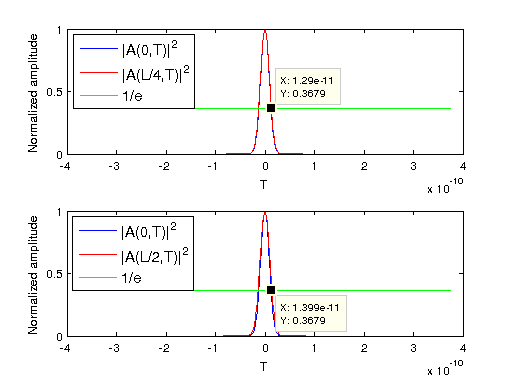
\includegraphics[width=11cm]{es2_c00.png}\\
  \caption{Values of $T_1$ for C=0.}
  \label{es2_C00}
\end{figure}

\begin{figure}[!ht]
  \centering
  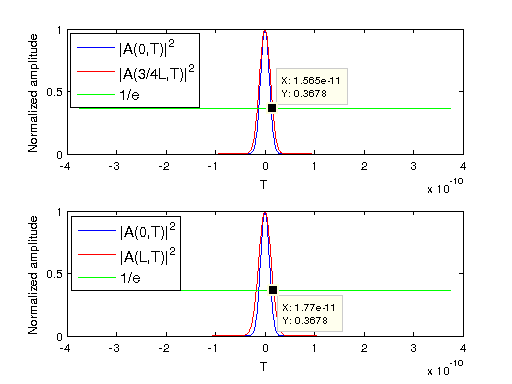
\includegraphics[width=11cm]{es2_c01.png}\\
  \caption{Values of $T_1$ for C=0.}
  \label{es2_C01}
\end{figure}

\begin{figure}[!ht]
  \centering
  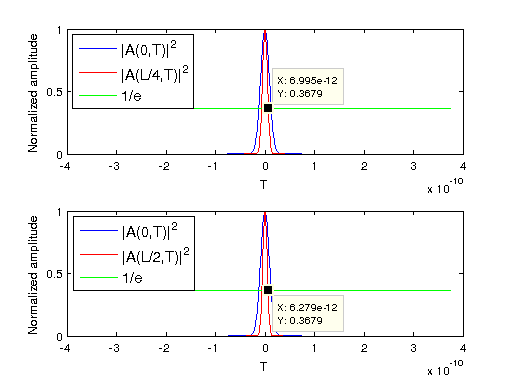
\includegraphics[width=11cm]{es2_c21.png}\\
  \caption{Values of $T_1$ for C=2.}
  \label{es2_C21}
\end{figure}

\begin{figure}[!ht]
  \centering
  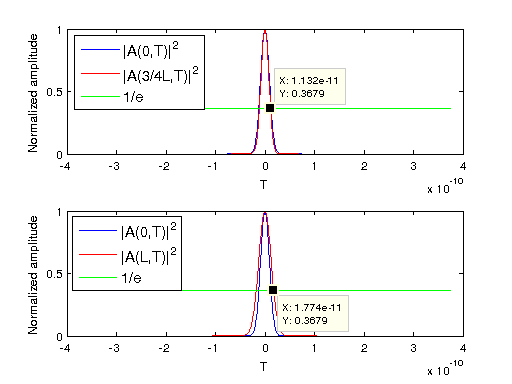
\includegraphics[width=11cm]{es2_c22.png}\\
  \caption{Values of $T_1$ for C=2.}
  \label{es2_C22}
\end{figure}

\begin{figure}[!ht]
  \centering
  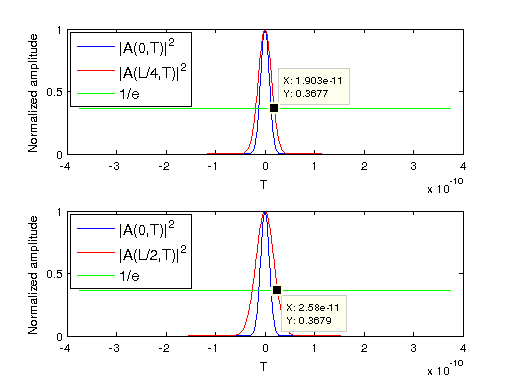
\includegraphics[width=11cm]{es2_cm21.png}\\
  \caption{Values of $T_1$ for C=-2.}
  \label{es2_Cm21}
\end{figure}

\begin{figure}[!ht]
  \centering
  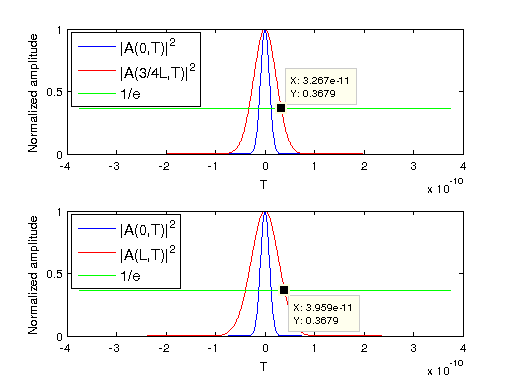
\includegraphics[width=11cm]{es2_cm22.png}\\
  \caption{Values of $T_1$ for C=-2.}
  \label{es2_Cm22}
\end{figure}

\begin{figure}[!ht]
  \centering
  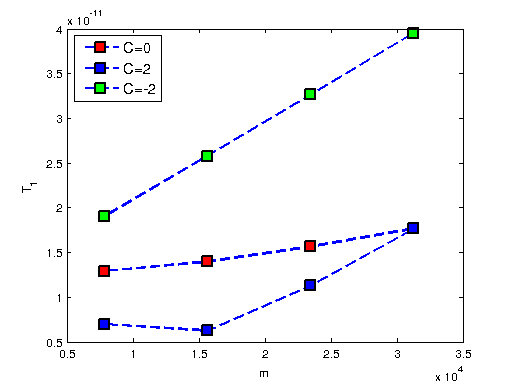
\includegraphics[width=11cm]{es2_plot.png}\\
  \caption{Values of $T_1$ versus length, for C=0, 2 and -2.}
  \label{es2_plot}
\end{figure}

\newpage
In Figure \ref{es2_plot} are reported the measured values of $T_1$ versus the length.
As we can observe, if the chirp is absent, the pulse broadens slowly and linearly with the distance (red dots).
If the initial chirp is positive (blue dots), the pulse shrinks for the first 16 Km and then starts broadening. At the end of the propagation,
the value $T_1(L)$ is identical to the case with C=0. 
When the initial chirp is negative (green dots), the pulse broadens linearly with the distance, but with a higher slope respect to the case with C=0.

Now we repeat the same simulation, changing the sign of the dispersion ($\beta_2 = 5 \cdot 10^{-27} \ [s^2/m]$).
In Figure \ref{es2_plot2} is shown the result.
\begin{figure}[!ht]
  \centering
  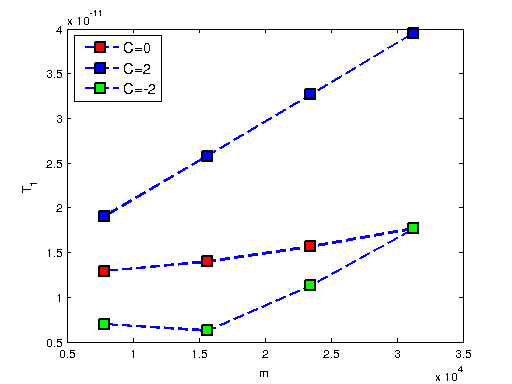
\includegraphics[width=11cm]{es2_plot2.png}\\
  \caption{Values of $T_1$ versus length, for C=0, 2 and -2 and positive dispersion.}
  \label{es2_plot2}
\end{figure}
The curve with C=0 remains unchanged, while the other two curves are the opposite respect to the case with negative beta.

\newpage
%%%%%%%%%%%%%%%%%%%%%%%%%%%%%%%%%%%%%%%%%%%%%%%%%%%%%%%%%%%%%%%%%%%%%%%%%%%%%%%%%%%%%%%%%%%%%%
\section*{Exercise 3}
We set the dispersion to zero and the attenuation to 0.2 dB/Km.
We propagate the pulse of equation (\ref{pulse}) for 40 Km and we verify that, the pulse peak power at the end
of the simulation, has decreased by 8 dB.
The power attenuation relationship is: 
$$P(L)=P(0) \cdot e^{-\alpha L}$$

The amplitude of a signal is proportional to the square root of its power, so:
\begin{equation}\label{power}
A(L)=\sqrt{P(0) \cdot e^{-\alpha L}}=A(0) \cdot e^{-\frac{\alpha L}{2}}
\end{equation}
But $\alpha$ is expressed in linear units, while our attenuation is given in dB.
So we have to convert it:
$$\alpha_{dB}=-10 \log \left(\frac{P_o}{P_i} \right)=-10 \log \left(\frac{P(0) e^{-\alpha}}{P(0)} \right) = -10 \log \left( e^{-\alpha} \right)$$
and we invert the equation to extract $\alpha$:
$$\alpha=\alpha_{linear}=-\ln \left( 10^{-\frac{\alpha_{dB}}{10}}\right)$$
We substitute in the above equation $\alpha_{dB}=0.2 \cdot 10^{-3}\ [dB/m]$ and we obtain the equivalent linear coefficient:
$$\alpha=4.6052\cdot10^{-5} \ [1/m]$$
To find the total attenuation we substitute this value and the length into the equation (\ref{power}) and we obtain:
$$A(L)=A(0) \cdot e^{-\frac{\alpha L}{2}}=A(0) \cdot 0.3981$$
So, after a length of 40000 meters, the pulse is attenuated by a factor 0.3981.
This is confirmed by the simulation we have run: in Figure \ref{es3} is shown the pulse in time at the beginning of the propagation (in blue)
and at the end of the propagation (in red). The respectively maximums are $A(0)_{max}=0.9995$ and $A(L)_{max}=0.3979$.
The ratio $A(L)_{max}/A(0)_{max}=0.3981$ corresponds exactly to the theoretical attenuation.

\begin{figure}[!ht]
  \centering
  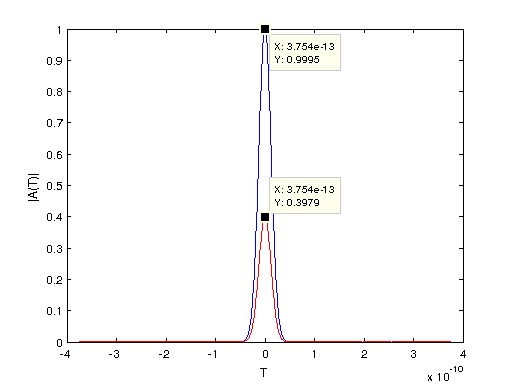
\includegraphics[width=11cm]{es3.png}\\
  \caption{Shape of $|A(T)|$ at the beginning and at the end of propagation.}
  \label{es3}
\end{figure}

\newpage
%%%%%%%%%%%%%%%%%%%%%%%%%%%%%%%%%%%%%%%%%%%%%%%%%%%%%%%%%%%%%%%%%%%%%%%%%%%%%%%%%%%%%%%%%%%%%%
\section*{Exercise 4}
Now we introduce in the simulation Kerr non-linearities. We set $\gamma = 2\cdot 10^{-3} \ [W^{-1}m^{-1}]$ and
$\beta_2=0$. We plot the phase profile for three different values of power: $P_1=50 \ mW$, $P_2=100 \ mW$ and $P_3=150 \ mW$.
In Figure \ref{phase1} is shown the phase of the pulse at the end of propagation.

\begin{figure}[!ht]
  \centering
  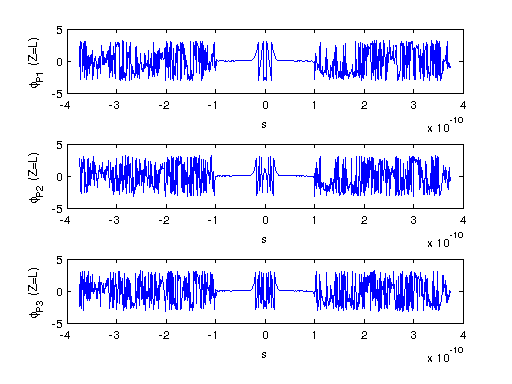
\includegraphics[width=11cm]{es4_phaseb0.png}\\
  \caption{Phase profile for P1, P2, P3 and zero dispersion.}
  \label{phase1}
\end{figure}

We then run the simulation introducing a dispersion value of $\beta_2 = -5 \cdot 10^{-27} \ [s^2/m]$ and setting $\gamma = 0$.
In Figure \ref{phase3} are shown the results.
\begin{figure}[!ht]
  \centering
  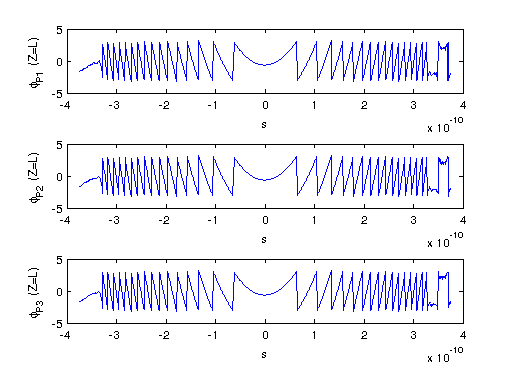
\includegraphics[width=11cm]{es4_phasebnogam.png}\\
  \caption{Phase profile for P1, P2, P3 and zero non-linearities.}
  \label{phase3}
\end{figure}

When we have non-linearities also the phase has a non linear behaviour that is proportional to the power of the pulse.
Instead, when non-linearities are absent and we introduce dispersion, the phase is quasi linear and it doesn't change for the different powers.

\newpage
Now we observe the behaviour of the absolute value of the pulse spectrum, as a function of the propagation distance, for different input power values.
We use the same power values of before and we set a length of $L=10^5\ m$. The non-linear coefficient is $\gamma = 2\cdot 10^{-3} \ [W^{-1}m^{-1}]$.
The spectrum of the propagated signal exhibits a number of peaks M, that depends upon the following relationship: $$\gamma P L \approx (M-0.5)\pi$$
and so:$$M \approx 0.5 + \frac{\gamma P L}{\pi}$$
Substituting the values of the three powers, we obtain:
\begin{itemize}
 \item $M_1 \approx 4$
 \item $M_2 \approx 7$
 \item $M_3 \approx 10$
\end{itemize}


In Figure \ref{powers} is shown the result of the simulation. It is plotted the module of the FFT of the pulse, at the end of propagation.
The estimated number of peaks, coincides with the ones obtained in the simulation.
\begin{figure}[!ht]
  \centering
  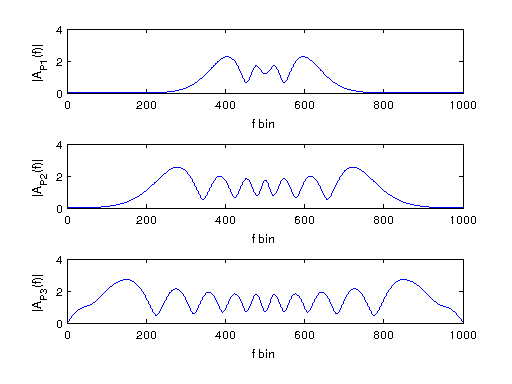
\includegraphics[width=11cm]{es4_powers.png}\\
  \caption{Peaks due to different peak powers.}
  \label{powers}
\end{figure}


%%%%%%%%%%%%%%%%%%%%%%%%%%%%%%%%%%%%%%%%%%%%%%%%%%%%%%%%%%%%%%%%%%%%%%%%%%%%%%%%%%%%%%%%%%%%%%
\section*{Exercise 5}
We study the propagation of solitons. A soliton is a pulse with the following shape:
$$A(T)=N \sqrt{\frac{|\beta_2|}{\gamma {T_0}^2}} sech \left( \frac{T}{T_0}\right)$$
We set the parameters:
\begin{itemize}
 \item N=1
 \item $\beta_2 = -15 \cdot 10^{-27} \ [s^2/m]$
 \item $\gamma = 2 \cdot 10^{-3} \ [W^{-1} m^{-1}]$
 \item $T_0=1.25 \cdot 10^{-11} \ s$
 \item $L=10^5 \ m$
\end{itemize}

In Figure \ref{soliton} is shown the propagation of a soliton with the above characteristics. We can observe that it propagates unchanged
in presence of dispersion and non-linearities.
In fact the non linear effect tends to shrink the pulse, while the dispersion tends to enlarge it.
The non linear effect compensates the dispersion and the pulse propagates without widening.

\begin{figure}[!ht]
  \centering
  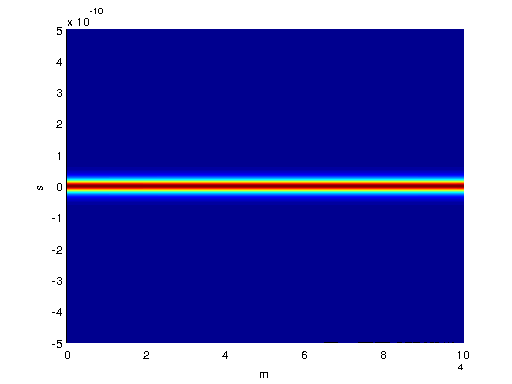
\includegraphics[width=11cm]{es5_soliton.png}\\
  \caption{Propagation of a soliton (top view).}
  \label{soliton}
\end{figure}

Now we increase the power by setting N=3, in Figure \ref{es5_N3} is shown the result.
\begin{figure}[!ht]
  \centering
  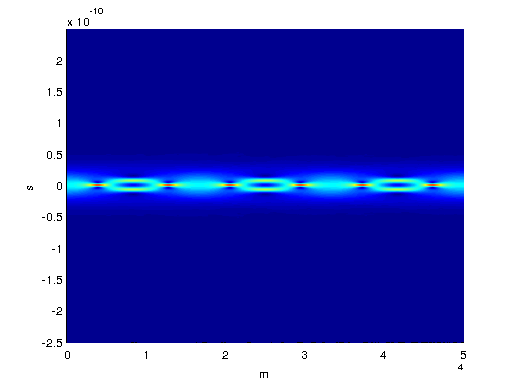
\includegraphics[width=11cm]{es5_N3.png}\\
  \caption{Propagation of a soliton with N=3.}
  \label{es5_N3}
\end{figure}

The evolution is periodic, the peaks are in the positions:
$$Z=[0.39,   1.27,  2.05,   2.93,  3.70,   4.57,   5.37,   6.25, 6.87, 7.01,  7.88, 8.62, 9.41]\cdot 10^4 \ m$$
The average of the peak periods is $\Delta T_1=8208 \ m$.
Now we reduce the power of $10 \%$ and we observe the behaviour of the peaks. In Figure \ref{es5_N27} is shown the result.
\begin{figure}[!ht]
  \centering
  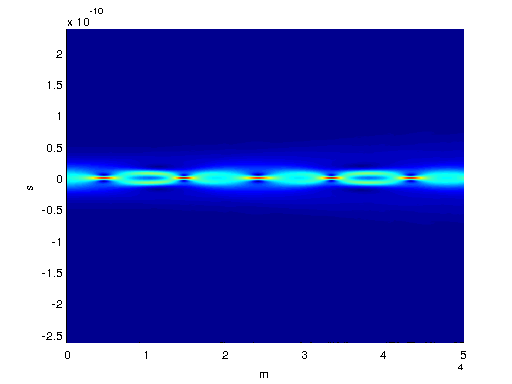
\includegraphics[width=11cm]{es5_N27.png}\\
  \caption{Propagation of a soliton with N=2.7.}
  \label{es5_N27}
\end{figure}
The average period is now $\Delta T_2=9529 \ m$.

We increase the power of $10 \%$ and in Figure \ref{es5_N33} we can observe the result: the average period is $\Delta T_3= 3097 \ m$.

\begin{figure}[!ht]
  \centering
  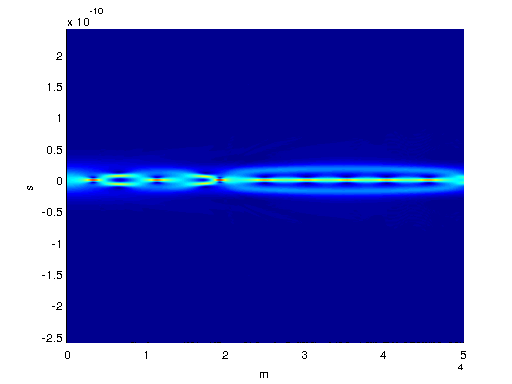
\includegraphics[width=11cm]{es5_N33.png}\\
  \caption{Propagation of a soliton with N=3.3.}
  \label{es5_N33}
\end{figure}
We can conclude that, increasing the power, the period of the peaks decreases and vice versa.

If we change the sign of beta, the propagation is modified: in Figure \ref{es5_positivebeta} is shown the propagation for N=1.
The effect of dispersion and non-linear effect act in phase and so the pulse is dispersed.

\begin{figure}[!ht]
  \centering
  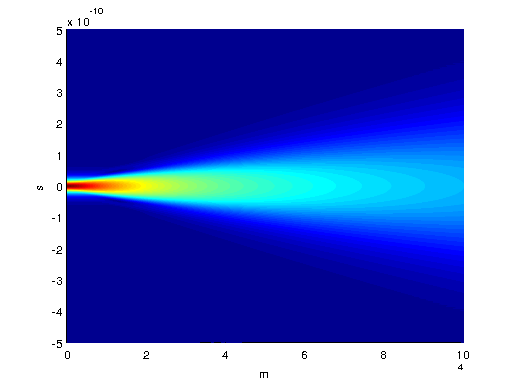
\includegraphics[width=11cm]{es5_positivebeta.png}\\
  \caption{Propagation of a soliton with N=1 and positive beta.}
  \label{es5_positivebeta}
\end{figure}
\newpage
Now we propagate a Gaussian pulse with the same characteristics of the soliton (non-linearities and positive dispersion),
in Figure \ref{es5_gauss} is shown the propagation result. The Gaussian pulse is dispersed faster than the soliton.

\begin{figure}[!ht]
  \centering
  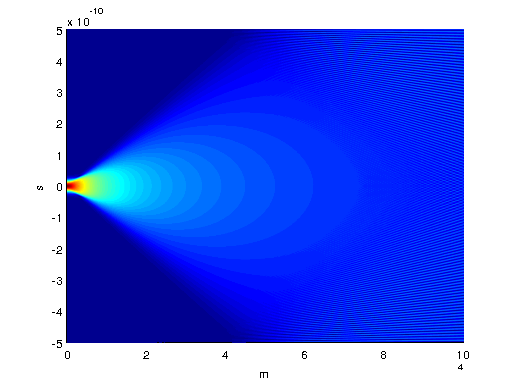
\includegraphics[width=11cm]{es5_gauss.png}\\
  \caption{Propagation of a Gaussian pulse with N=1 and positive beta.}
  \label{es5_gauss}
\end{figure}

\newpage
%%%%%%%%%%%%%%%%%%%%%%%%%%%%%%%%%%%%%%%%%%%%%%%%%%%%%%%%%%%%%%%%%%%%%%%%%%%%%%%%%%%%%%%%%%%%%%
\section*{Exercise 6}
We launch two successive soliton pulses, with the center position shifted in time by $K T_0$, with K=5 and simulation length $2\cdot 10^6 \ m$.
The result is shown in Figure \ref{es6_1}.
The pulses start separately in time but, during propagation, they attract each other and so, there are points in which they hit and create a peak.
Measuring the peak distance, we find the average value of the period: $\Delta T=39319 \ m$.

\begin{figure}[!ht]
  \centering
  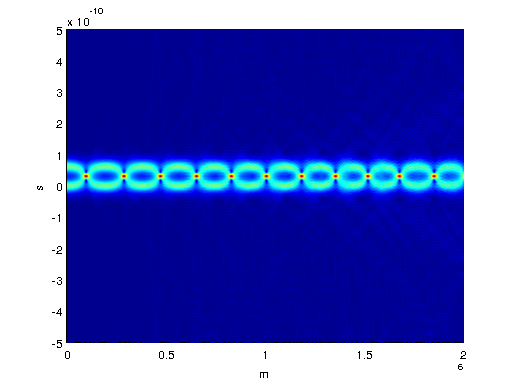
\includegraphics[width=11cm]{es6_1.png}\\
  \caption{Propagation of two solitons shifted in time (K=5).}
  \label{es6_1}
\end{figure}

We set now K=8 and in Figure \ref{es6_2} we see the result.
\begin{figure}[!ht]
  \centering
  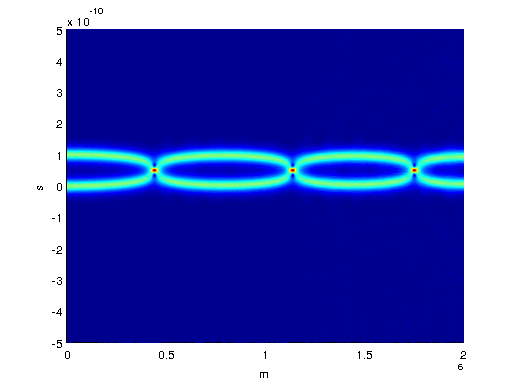
\includegraphics[width=11cm]{es6_2.png}\\
  \caption{Propagation of two solitons shifted in time (K=8).}
  \label{es6_2}
\end{figure}
The average distance between peaks now is increased: in fact it is $\Delta T=71214 \ m$.

Now we shift the phase of the second pulse by $\pi$, in Figure \ref{es6_3} is shown the result.
\begin{figure}[!ht]
  \centering
  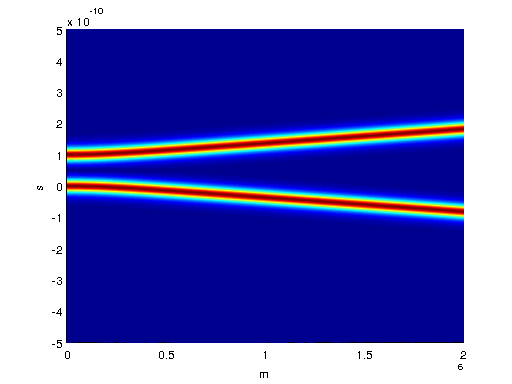
\includegraphics[width=11cm]{es6_3.png}\\
  \caption{Propagation of two solitons shifted in time (K=5) and with opposite phase.}
  \label{es6_3}
\end{figure}

The two pulses propagate without hitting one with each other. This is due to the fact that, having opposite phases,
they are more distant and so they don't attract each other. Instead they modify their propagation velocity.

These factors are important when transmitting train of pulses: if they are in phase they attract each other causing some hits,
which period is proportional to the time shift between pulses.
When they are out of phase they don't hit, but they change their velocity.

\newpage
%%%%%%%%%%%%%%%%%%%%%%%%%%%%%%%%%%%%%%%%%%%%%%%%%%%%%%%%%%%%%%%%%%%%%%%%%%%%%%%%%%%%%%%%%%%%%%
\section*{Exercise 7}
We propagate a Gaussian pulse with the following characteristics:
\begin{itemize}
 \item Peak power = +6 dBm
 \item C=0
 \item $T_0=1.25 \cdot 10^{-11} \ s$
\end{itemize}
the power in linear units is $P=0.001 \cdot 10^{\frac{dBm}{10}}=4 \ mW$ and so the pulse amplitude is $A=\sqrt{P}=0.0631$.

The fiber has properties:
\begin{itemize}
 \item $\beta_2 = -20 \cdot 10^{-27} \ [s^2/m]$
 \item $\gamma = 2 \cdot 10^{-3} \ [W^{-1} m^{-1}]$
 \item $L=100 \ Km$
\end{itemize}

In Figure \ref{es7_1} is shown the simulation result.
\begin{figure}[!ht]
  \centering
  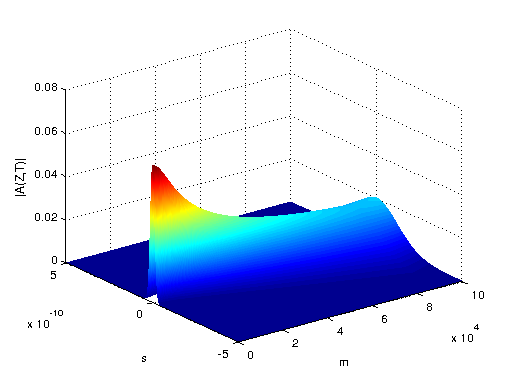
\includegraphics[width=11cm]{es7_1.png}\\
  \caption{Gaussian pulse.}
  \label{es7_1}
\end{figure}

Now we propagate the same pulse in a link composed of 4 spans (of length equal to 25 Km each), changing the sign of dispersion
at each span. In Figure \ref{es7_22} is shown the result.

\begin{figure}[!ht]
  \centering
  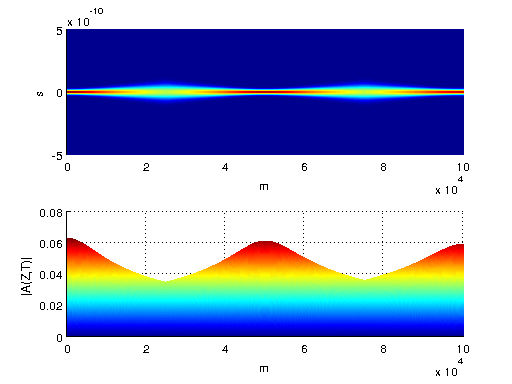
\includegraphics[width=11cm]{es7_22.png}\\
  \caption{Gaussian pulse with sign of dispersion changed every 25 Km.}
  \label{es7_22}
\end{figure}

When the sign of the dispersion is changed, the effect of the dispersion on the pulse is changed too, and so we have a reconstruction of the pulse.
In Figure \ref{es7_3} is shown the pulse at the beginning (blue line) and at the end of the fiber (red line), in time and frequency domain.
\begin{figure}[!ht]
  \centering
  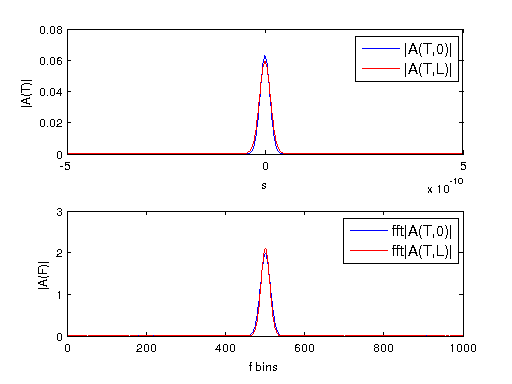
\includegraphics[width=11cm]{es7_3.png}\\
  \caption{Gaussian pulse with sign of dispersion changed every 25 Km.}
  \label{es7_3}
\end{figure}

We can observe that, the shape of the pulse at the end of the fiber, is almost identical to the shape at the beginning of the fiber (in time and
in frequency domain). This is because, at the end of the propagation, the dispersion is fully compensated.

\newpage
Now we simulate the propagation through a 100 Km length link, with the first 90 Km with $\beta_2 = -20 \cdot 10^{-27} \ [s^2/m]$
and the last 10 Km with a beta that compensates the accumulated dispersion.
The relationship that relates dispersions and lengths is: $$L_1 D_1 = -L_2 D_2$$
and so: $$D_2=-\frac{L_1}{L_2}D_1=-9 D_1$$
In Figure \ref{es7_comp2} and \ref{es7_comp3} is shown the simulation result.


\begin{figure}[!ht]
  \centering
  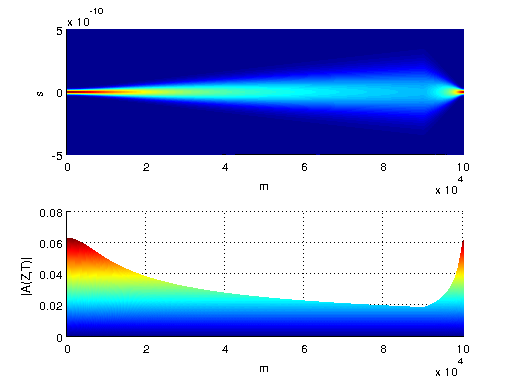
\includegraphics[width=11cm]{es7_comp2.png}\\
  \caption{Gaussian pulse with total compensation after 90 Km.}
  \label{es7_comp2}
\end{figure}

\begin{figure}[!ht]
  \centering
  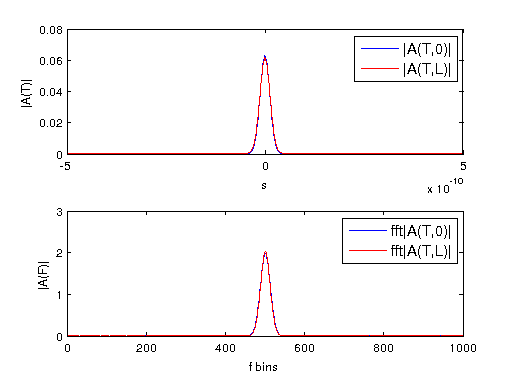
\includegraphics[width=11cm]{es7_comp3.png}\\
  \caption{Gaussian pulse with total compensation after 90 Km.}
  \label{es7_comp3}
\end{figure}

We have again a total reconstruction of the pulse, because we compensated the dispersion, even if in an asymmetrical mode
respect to the previous case. In the second span the dispersion value is higher, so the desired reconstruction happens in a shorter distance.
In this second case, the pulse broadening is higher respect to the previous one and this can create interference problems
when transmitting train of pulses.


\newpage
%%%%%%%%%%%%%%%%%%%%%%%%%%%%%%%%%%%%%%%%%%%%%%%%%%%%%%%%%%%%%%%%%%%%%%%%%%%%%%%%%%%%%%%%%%%%%%
\section*{Exercise 8}
We propagate a Gaussian pulse in a fiber the following characteristics:
\begin{itemize}
 \item $\beta_2 = -10 \cdot 10^{-27} \ [s^2/m]$
 \item $\gamma = 2 \cdot 10^{-3} \ [W^{-1} m^{-1}]$
 \item $L=7 \cdot 10^4 \ m$
\end{itemize}

The pulse has:
\begin{itemize}
 \item Peak power = +3 dBm
 \item C=0
 \item $T_0=1.25 \cdot 10^{-11} \ s$
\end{itemize}
along with that, are injected in the fiber other two pulses with the same characteristics, but with frequency shifts of $\Delta f=100 \ GHz$
and $\Delta f = -100 \ GHz$.
In Figure \ref{es8_1} and \ref{es8_2} is represented the simulation in time domain and in Figure \ref{es8_f1} the spectrum at the beginning
and at the end of the propagation.

\begin{figure}[!ht]
  \centering
  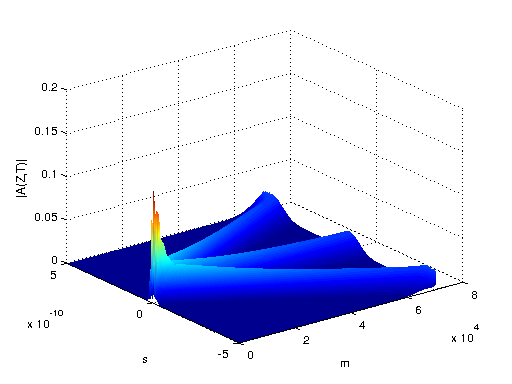
\includegraphics[width=11cm]{es8_1.png}\\
  \caption{Gaussian pulses with frequency shift.}
  \label{es8_1}
\end{figure}

\begin{figure}[!ht]
  \centering
  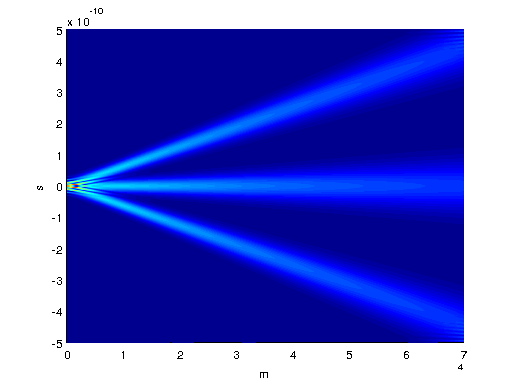
\includegraphics[width=11cm]{es8_2.png}\\
  \caption{Gaussian pulses with frequency shift (top view).}
  \label{es8_2}
\end{figure}

\begin{figure}[!ht]
  \centering
  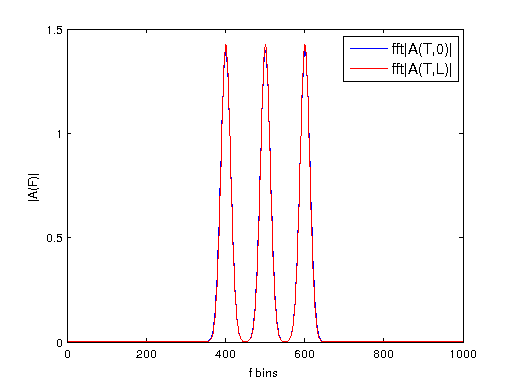
\includegraphics[width=11cm]{es8_f1.png}\\
  \caption{Gaussian pulses with frequency shift in frequency domain.}
  \label{es8_f1}
\end{figure}


The pulse with negative frequency shift decreases its velocity, while the one with positive shift increases the velocity.
The spectra at the beginning and at the end of the propagation have the same shape.

We now set the value of the dispersion to $\beta_2 = -1 \cdot 10^{-27} \ [s^2/m]$ and we run the same simulation.
In Figure \ref{es8_3}, \ref{es8_4} and \ref{es8_f2} are shown the results.
Again, the velocities of the shifted pulses are changed, but the values are smaller respect to the previous case.
The spectra at the beginning and at the end of the simulation remain unchanged.

\begin{figure}[!ht]
  \centering
  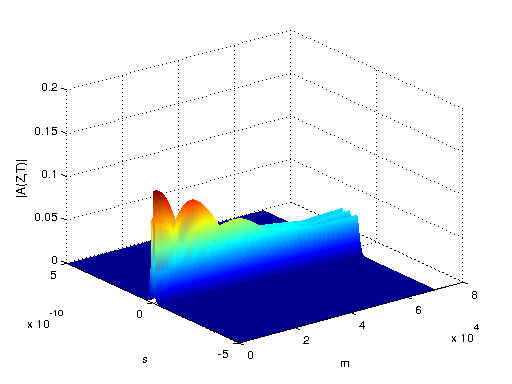
\includegraphics[width=11cm]{es8_3.png}\\
  \caption{Gaussian pulses with frequency shift.}
  \label{es8_3}
\end{figure}

\begin{figure}[!ht]
  \centering
  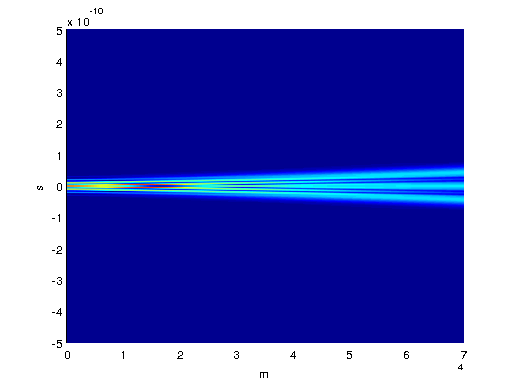
\includegraphics[width=11cm]{es8_4.png}\\
  \caption{Gaussian pulses with frequency shift (top view).}
  \label{es8_4}
\end{figure}

\begin{figure}[!ht]
  \centering
  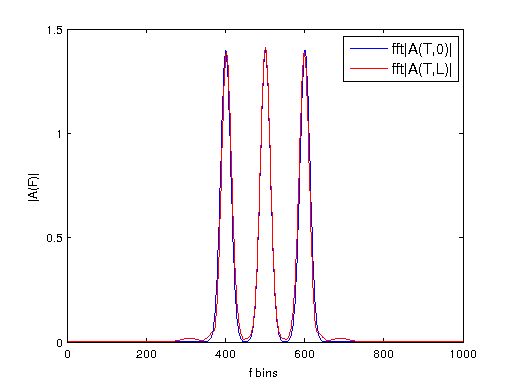
\includegraphics[width=11cm]{es8_f2.png}\\
  \caption{Gaussian pulses with frequency shift in frequency domain.}
  \label{es8_f2}
\end{figure}

\end{document}




